% DEFINING COLORS COF, PUR, GREEO AND GREET
\definecolor{cof}{RGB}{219,144,71}
\definecolor{pur}{RGB}{186,146,162}
\definecolor{greeo}{RGB}{91,173,69}
\definecolor{greet}{RGB}{52,111,72}
% CUBE
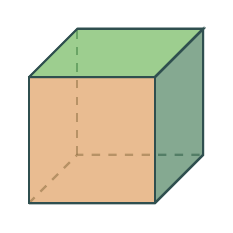
\begin{tikzpicture}[thick,scale=0.8,DarkSlateGray]
    \coordinate (A1) at (-1,-1,-1);
    \coordinate (A2) at (-1,-1,1);
    \coordinate (A3) at (-1,1,-1);
    \coordinate (A4) at (-1,1,1);
    \coordinate (B1) at (1,-1,-1);
    \coordinate (B2) at (1,-1,1);
    \coordinate (B3) at (1,1,-1);
    \coordinate (B4) at (1,1,1);
    %
    % Drawing dashed lines
    \begin{scope}[thick,dashed,opacity=0.6]
        \draw (A2) -- (A1) -- (B1);
        \draw (A1) -- (A3);
    \end{scope}
    %
    % Color Faces
    \draw[fill=cof,opacity=0.6]   (A4) -- (B4) -- (B2) -- (A2) ;
    \draw[fill=greet,opacity=0.6]   (B4) -- (B3) -- (B1) -- (B2) ;
    \draw[fill=greeo,opacity=0.6] (A4) -- (B4) -- (B3) -- (A3) ;
    %
    % Drawing Edges
    \draw (A2) -- (B2) -- (B1) ;
    \draw (A2) -- (A4) -- (B4) -- (B2) -- cycle ;
    \draw (A4) -- (A3) -- (B3) -- (B4) ;   
    \draw (B3) -- (B1);
    %
\end{tikzpicture}